\documentclass[11pt, a4paper]{article}

% =============================================================================
% Preamble
% =============================================================================
\usepackage[margin=2.4cm, headheight=15pt]{geometry}
\usepackage{microtype}
\usepackage{parskip}

\usepackage{amsmath, amssymb, mathtools}
\usepackage{booktabs}
\usepackage{tabularx}
\usepackage{array}
\usepackage{graphicx}
\usepackage{caption}
\usepackage{enumitem}
\usepackage{listings}
\usepackage{mdframed}
\usepackage{xcolor}
\usepackage{titlesec}
\usepackage{fancyhdr}

\definecolor{headerblue}{RGB}{0,70,127}
\definecolor{noteblue}{RGB}{220,235,245}
\definecolor{warnyellow}{RGB}{255,248,220}
\definecolor{codegrey}{RGB}{245,245,245}
\definecolor{accent}{RGB}{138,75,45}

\usepackage{hyperref}
\hypersetup{
  colorlinks = true, linkcolor = headerblue, urlcolor = headerblue,
  citecolor = headerblue,
  pdftitle = {Kala Chakra: KP Horary Automation},
  pdfauthor = {Amriit Mohapatra}
}

\titleformat{\section}{\large\bfseries\color{headerblue}}{\thesection}{0.6em}{}[\titlerule]
\titleformat{\subsection}{\normalsize\bfseries\color{headerblue!80}}{\thesubsection}{0.5em}{}
\titleformat{\subsubsection}{\normalsize\itshape}{\thesubsubsection}{0.5em}{}

\pagestyle{fancy}
\fancyhf{}
\rhead{\small Kala Chakra --- KP Horary Automation}
\lhead{\small Technical Documentation}
\rfoot{\small Page \thepage}
\lfoot{\small \c{k}\=ala cakra}
\renewcommand{\headrulewidth}{0.4pt}

\newmdenv[backgroundcolor=noteblue, linecolor=headerblue, linewidth=1pt,
  roundcorner=4pt, innerleftmargin=10pt, innerrightmargin=10pt,
  innertopmargin=8pt, innerbottommargin=8pt]{notebox}
\newmdenv[backgroundcolor=warnyellow, linecolor=orange!70, linewidth=1pt,
  roundcorner=4pt, innerleftmargin=10pt, innerrightmargin=10pt,
  innertopmargin=8pt, innerbottommargin=8pt]{warnbox}

\lstset{
  basicstyle = \small\ttfamily, keywordstyle = \color{headerblue}\bfseries,
  commentstyle = \color{gray}\itshape, breaklines = true, frame = single,
  framesep = 4pt, rulecolor = \color{gray!40}, backgroundcolor = \color{codegrey}
}

\newcommand{\code}[1]{\texttt{#1}}

% =============================================================================
\begin{document}
% =============================================================================

\begin{titlepage}
  \centering
  \vspace*{1.6cm}
  {\Large\bfseries\color{headerblue} Kala Chakra \quad(\textnormal{\itshape k\=ala cakra})}\\[0.4em]
  {\normalsize The Wheel of Time --- Odia: written \textit{k\=ala cakra}}
  \vspace{1.3cm}

  \rule{\textwidth}{1.5pt}\\[0.5em]
  {\LARGE\bfseries Automating the KP Horary Workflow}\\[0.4em]
  {\large From raw astrological export to star/sub lords, cusp numbers,\\
   and the step-wise power calculation}\\
  \rule{\textwidth}{1.5pt}
  \vspace{1.3cm}

  \begin{tabular}{ll}
    \textbf{Author:}   & Amriit Mohapatra \\
    \textbf{Method:}   & Krishnamurti Paddhati (KP), East Indian style \\
    \textbf{Deliverables:} & Python package, JavaScript app, Excel pipeline \\
    \textbf{Date:}     & \today \\
  \end{tabular}
  \vfill

  \begin{notebox}
  \small This document describes the computational method exactly as
  implemented. Every rule was reconstructed from the author's manual
  workflow (the \code{Guide\_Step1}--\code{Guide\_Step6} sheets and hand-drawn
  notes) and validated against a corpus of previously hand-calculated
  charts. It is intended as a durable reference for future maintenance and
  debugging.
  \end{notebox}
\end{titlepage}

\tableofcontents
\newpage

% =============================================================================
\section{Introduction}
% =============================================================================

Horary astrology answers a specific question --- ``Will I get this job?'',
``Will the admission come through?'' --- from a chart cast for the moment the
question is posed, at a given place and time. Under Krishnamurti Paddhati
(KP), the answer is read not from the signs alone but from a nested lordship
scheme: each point in the zodiac has a \emph{star lord} (the ruler of its
nakshatra) and a \emph{sub lord} (a finer subdivision), and the relationships
between the planets, their lords, and the twelve house cusps are combined into
a numeric ``power'' expression that the astrologer interprets.

Performed by hand, one chart takes 15--25 minutes of careful table lookups and
arithmetic, and the work is error-prone: a single mis-read table row or an
off-by-one house boundary silently corrupts everything downstream. \textbf{Kala
Chakra} automates the entire sequence, reducing a chart to 2--3 minutes with no
arithmetic slips, while showing every intermediate step so the astrologer
retains full interpretive control.

\begin{notebox}
\textbf{Scope.} The system automates everything up to and including the power
calculation. It does \emph{not} interpret the result or cast dasha periods ---
those remain the astrologer's work. Planetary and cuspal longitudes are taken
as given from professional astrology software; Kala Chakra does not compute
ephemerides.
\end{notebox}

% =============================================================================
\section{The Six-Step Manual Workflow}
% =============================================================================

The automation mirrors the author's own six-step process, so that each block
can be checked against the manual method it replaces.

\begin{enumerate}[leftmargin=1.4em]
  \item \textbf{Capture the raw chart.} The astrology software (Solar Fire)
    produces a \textsc{Chart Analysis Report}: house cusps and planetary
    longitudes in degrees, minutes and seconds, plus a large amount of
    unrelated material.
  \item \textbf{Clean and lay out.} Keep only the twelve cusps and nine KP
    points. The node \code{Nod} is renamed \code{Ra} (Rahu); \code{Ke} (Ketu)
    is added at the same degree in the opposite sign. Retrograde markers are
    dropped. The retained points are arranged in the fixed East Indian chart
    layout.
  \item \textbf{Record the query context.} Date, time and location are noted
    at the centre of the chart.
  \item \textbf{Assign star and sub lords, placements and ownership.} For each
    cusp and planet, look up (here: \emph{compute}) the star lord and sub lord.
    Assign each planet the cusp it occupies, and the cusp numbers it owns.
  \item \textbf{Write the cusp-number vectors.} For each planet, an ordered
    vector [placement, ownership\ldots]; for the nodes, a special
    dispositor-based vector.
  \item \textbf{Power calculation.} Combine placements and lordships into a
    numerator/denominator ``power'' expression, merge like terms, and render
    the final ascending line for each planet.
\end{enumerate}

% =============================================================================
\section{The Computational Core}
% =============================================================================

\subsection{Exact arithmetic in arcseconds}

Every longitude is stored as an integer number of arcseconds from
$0^\circ$ Aries:
\[
  \lambda \;=\; 3600\,d \;+\; 60\,m \;+\; s \;+\; 108{,}000 \times (\text{sign index}),
  \qquad 0 \le \lambda < 1{,}296{,}000.
\]
Because all KP boundaries fall on exact arcsecond values, integer arithmetic
makes the computation exact --- there is no floating-point rounding anywhere in
the chain. A full circle is $1{,}296{,}000''$; a sign is $108{,}000''$; a
nakshatra is $48{,}000''$ ($13^\circ20'$).

\subsection{Star lord and sub lord from Vimshottari proportions}

The 27 nakshatras cycle through nine lords in the fixed Vimshottari order
Ketu, Venus, Sun, Moon, Mars, Rahu, Jupiter, Saturn, Mercury. The
\textbf{star lord} of a longitude is simply the lord of the nakshatra it falls
in:
\[
  \text{star lord} \;=\; \text{VIM}\big[\,\lfloor \lambda / 48{,}000 \rfloor \bmod 9\,\big].
\]

The \textbf{sub lord} subdivides each nakshatra in proportion to the
Vimshottari dasha years (Ke 7, Ve 20, Su 6, Mo 10, Ma 7, Ra 18, Ju 16, Sa 19,
Me 17; total 120). The width of a sub within a nakshatra is
\[
  \text{width}(\ell) \;=\; \frac{\text{years}(\ell)}{120}\times 48{,}000
  \;=\; 400 \times \text{years}(\ell)\ \text{arcseconds},
\]
and the subs run in Vimshottari order \emph{starting from the star lord}.
Walking these cumulative widths from the start of the nakshatra locates the
sub. Boundaries are half-open, $[\text{from}, \text{to})$, matching the printed
KP tables.

\begin{notebox}
\textbf{Key design decision.} The 249-subdivision KP table is \emph{generated},
not stored. It follows deterministically from nine integers (the dasha years),
so there is no lookup file to transcribe or keep in sync. The generated table
was checked row-by-row against the scanned reference tables, including the
author's father's handwritten Taurus corrections, with zero discrepancies.
\end{notebox}

\subsection{Placement and ownership}

\textbf{Placement.} House $h$ spans the arc from cusp $h$ to cusp $h{+}1$
(in zodiacal order). A planet at longitude $\lambda$ occupies house $h$ when
$(\lambda - c_h) \bmod 1{,}296{,}000 < (c_{h+1} - c_h) \bmod 1{,}296{,}000$.
This modular test handles the wrap-around at $0^\circ$ Aries and the case of
two cusps in one sign automatically.

\textbf{Ownership.} Each planet rules one or two signs
(Table~\ref{tab:lordship}); it owns the cusp numbers that fall in those signs.
When one sign contains two cusps, its lord owns both. When a sign contains
\emph{no} cusp (because a neighbouring sign holds two), the whole sign lies
inside a single house span, and its lord owns that house --- the
\textbf{span rule}. Charts triggering the span rule are flagged with an
informational note.

\textbf{Nodes.} Rahu and Ketu own no sign. They act through their
\emph{dispositor} (the lord of the sign they occupy). The cusp-number vector
for a node is
\[
  [\,\text{dispositor's placement},\ \text{node's placement},\ \text{dispositor's ownerships}\ldots\,].
\]

\begin{table}[htbp]
  \centering
  \caption{Sign lordship used throughout (traditional KP rulership).}
  \label{tab:lordship}
  \begin{tabularx}{0.92\textwidth}{l X}
    \toprule
    Planet & Signs owned \\
    \midrule
    Sun (Su)     & Leo \\
    Moon (Mo)    & Cancer \\
    Mars (Ma)    & Aries, Scorpio \\
    Mercury (Me) & Gemini, Virgo \\
    Jupiter (Ju) & Sagittarius, Pisces \\
    Venus (Ve)   & Taurus, Libra \\
    Saturn (Sa)  & Capricorn, Aquarius \\
    Rahu / Ketu  & None --- act through the dispositor \\
    \bottomrule
  \end{tabularx}
\end{table}

% =============================================================================
\section{The Power Calculation}
% =============================================================================

The power calculation is the crux of the method. For each planet we identify
its Star lord and Sub lord (of the \emph{planet}, not the cusp), and build a
fraction whose terms are cusp numbers raised to fixed powers. The general form,
transcribed from the author's notation, is

\begin{equation}
  (\text{Planet},\ \text{Star},\ \text{Sub})
  \;=\;
  \frac{(\text{Planet})^{2}(\text{own})^{1}\;-\;(\text{Star})^{4}(\text{own})^{3}\;-\;(\text{Sub})^{6}(\text{own})^{5}}
       {(\text{Star})^{7}(\text{Sub})^{10}\;-\;(\text{Star})^{8}(\text{Sub})^{11}\;-\;(\text{Star})^{9}(\text{Sub})^{12}}.
  \label{eq:power}
\end{equation}

The dashes separate three \emph{groups} on each line and are structural, not
subtraction. Concretely:

\subsection{Numerator --- three parts}

\begin{itemize}[leftmargin=1.4em]
  \item \textbf{Planet:} its placement cusp gets power 2; each cusp it owns gets
    power 1.
  \item \textbf{Star lord:} the star lord's placement cusp gets power 4; each
    cusp it owns gets power 3.
  \item \textbf{Sub lord:} the sub lord's placement cusp gets power 6; each cusp
    it owns gets power 5.
\end{itemize}

\subsection{Denominator --- lordship of the twelve cusps}

For the Planet, its Star lord, and its Sub lord in turn, scan all twelve cusps:

\begin{itemize}[leftmargin=1.4em]
  \item cusps of which the \textbf{Planet} is star lord get power 7; sub lord,
    power 10;
  \item cusps of which the \textbf{Star lord} is star lord get power 8; sub
    lord, power 11;
  \item cusps of which the \textbf{Sub lord} is star lord get power 9; sub
    lord, power 12.
\end{itemize}

\subsection{The twelve powers as one grid}

The twelve powers are not arbitrary. They form a $3\times2\times2$ grid: the
role (Planet, Star, Sub), the aspect (numerator = the point's own
placement/ownership; denominator = its lordship over cusps), and the sub-aspect
(placement/star-lordship vs.\ ownership/sub-lordship).

\begin{table}[htbp]
  \centering
  \caption{The complete power assignment. Reading the two columns of each
  block in order Planet, Star, Sub gives $2,1;\,4,3;\,6,5$ (numerator) and
  $7,10;\,8,11;\,9,12$ (denominator).}
  \label{tab:powers}
  \begin{tabularx}{\textwidth}{l l l l}
    \toprule
    Role & Numerator (placement / own) & \multicolumn{2}{l}{Denominator (star lord / sub lord of cusps)} \\
    \midrule
    Planet    & $2$ \ / \ $1$ & $7$  & $10$ \\
    Star lord & $4$ \ / \ $3$ & $8$  & $11$ \\
    Sub lord  & $6$ \ / \ $5$ & $9$  & $12$ \\
    \bottomrule
  \end{tabularx}
\end{table}

\begin{warnbox}
\textbf{Corrected source typo.} The \code{Guide\_Step6} sheet, cell B44, writes
the star-lord ownership rule as ``current cuspal position \ldots\ power 4'',
duplicating part~2(a). The worked example on \code{Sheet2} makes the intended
rule unambiguous: star-lord \emph{ownership} carries power~3. The
implementation follows the worked example, and this choice is confirmed by the
27/27 agreement with the hand-calculated charts (Section~\ref{sec:validation}).
\end{warnbox}

\subsection{Node exception}

When a node (Rahu or Ketu) appears as the Planet, Star, or Sub of a term, the
\emph{position} power is assigned to both the node's placement \emph{and} its
dispositor's placement, and the \emph{ownership} power to the dispositor's
owned cusps. This is the same dispositor substitution used for the cusp-number
vectors, applied inside each numerator part.

\subsection{Merging}

Finally, identical base numbers combine by \emph{adding} their powers --- first
within the numerator, then within the denominator, then across the two. The
result is a single line of \code{base}$^{\text{power}}$ terms in ascending base
order. The application shows this as four steps: substitute the cusp numbers,
collect the numerator, collect the denominator, and merge-and-sort across both.

% =============================================================================
\section{Worked Example}
% =============================================================================

Figure~\ref{fig:chart} shows the reference chart (``Test1'') laid out in East
Indian style, with each cusp and planet placed in its sign box and annotated
with its star/sub lord and, for planets, the occupied house.

\begin{figure}[htbp]
  \centering
  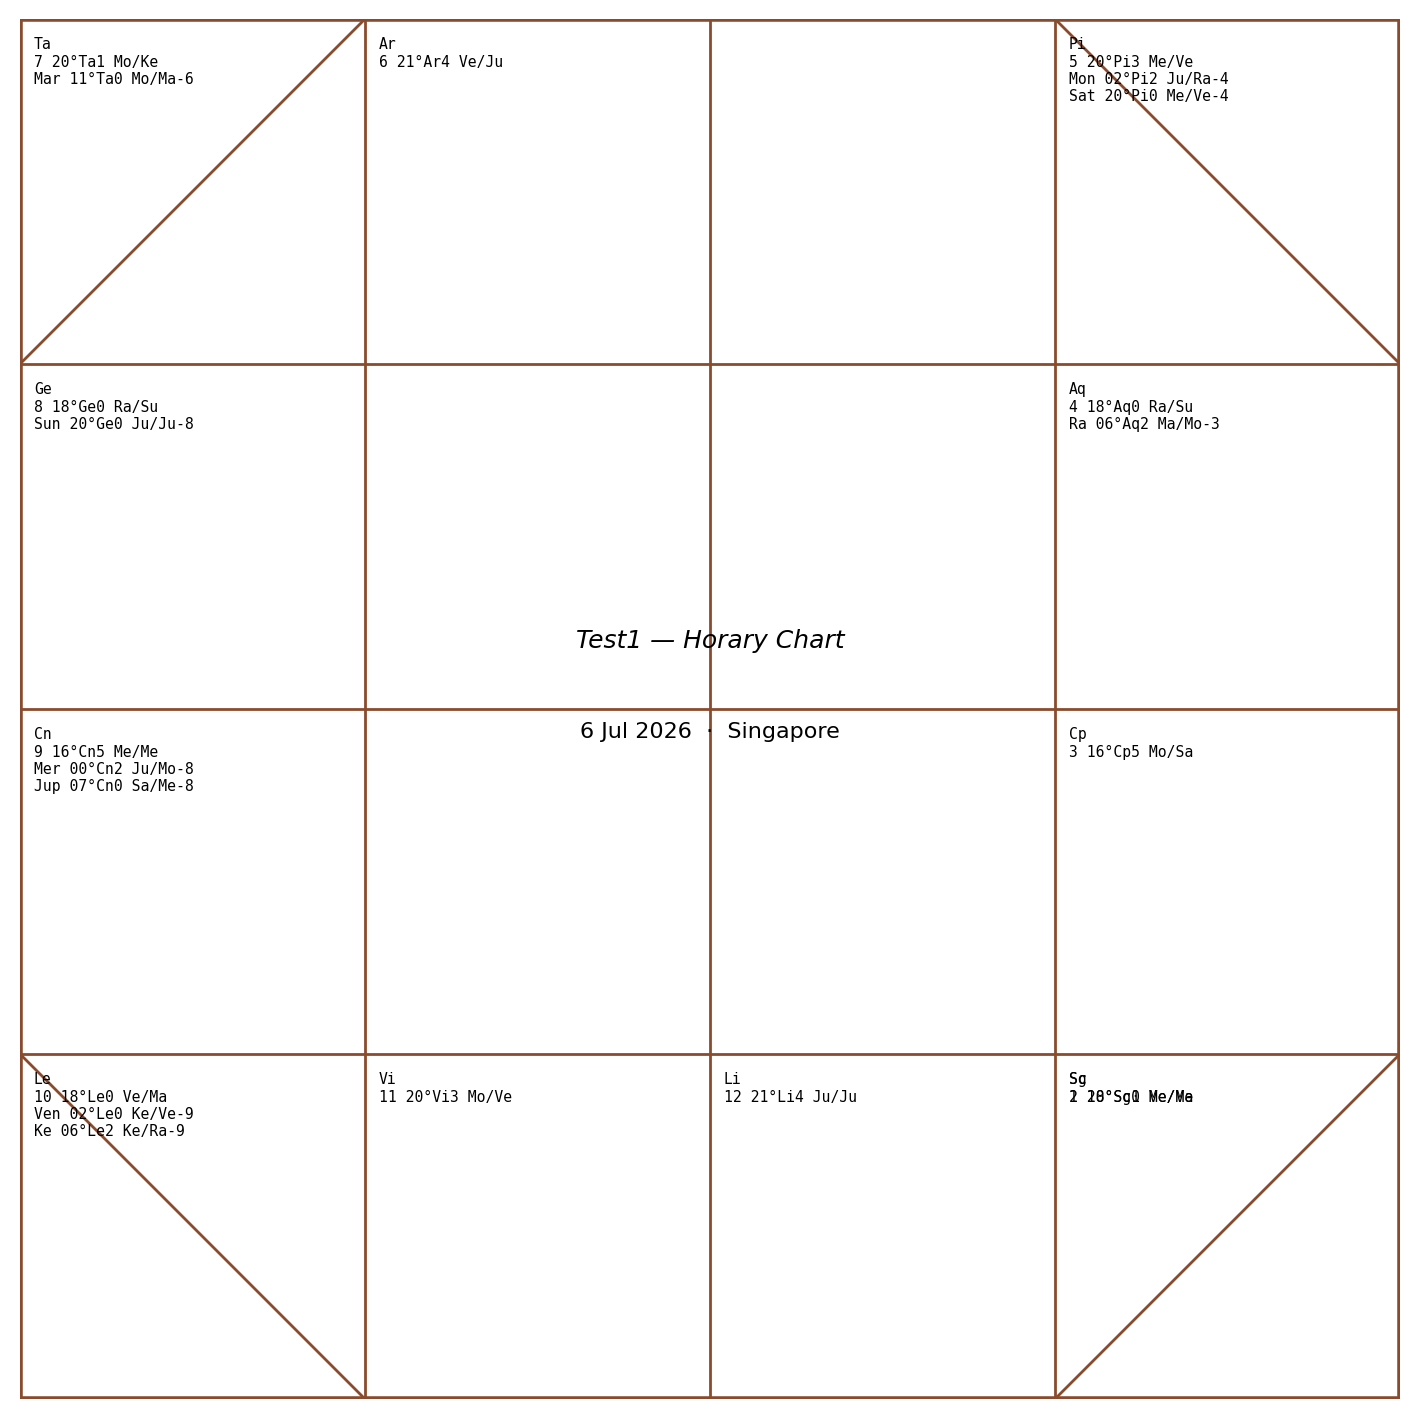
\includegraphics[width=0.86\textwidth]{figures/east_indian_chart.png}
  \caption{The reference chart rendered by Kala Chakra. Sign positions are
  fixed; cusp numbers and planets move with the moment of the query. Each entry
  reads \emph{number/name, longitude, star lord / sub lord}, with a trailing
  \emph{-house} tag for planets.}
  \label{fig:chart}
\end{figure}

Taking the Moon as an example: it lies at $02^\circ$Pi$28'13''$, whose star
lord is Jupiter and sub lord is Rahu, in house~4. Its cusp-number vector is
$4,9$ (placed in cusp~4, owns cusp~9). Running Equation~\eqref{eq:power} and
merging yields the final power line
\[
  2^{3}\ 3^{18}\ 4^{22}\ 5^{3}\ 6^{11}\ 7^{7}\ 8^{13}\ 9^{1}\ 11^{7}\ 12^{19},
\]
which matches the value obtained by hand. The application shows the full
substitution and both collection steps that lead here.

% =============================================================================
\section{Software Architecture}
% =============================================================================

\subsection{Two engines, one specification}

The method is implemented twice: once in Python (\code{kp\_core.py} and
helpers) and once in JavaScript (\code{web/kp\_logic.js}). The Python engine
drives the command-line tools and the Excel pipeline; the JavaScript engine
drives the browser app, which needs no installation. Both are held to the same
specification by a parity test that runs every chart through both and compares
every star lord, sub lord, house tag, cusp-number vector and power string.

\subsection{Style-safe Excel editing}

The East Indian chart in the output workbook is a real drawing --- twelve line
shapes. General-purpose spreadsheet libraries silently discard such drawings on
save. Kala Chakra therefore edits workbooks \emph{surgically}: it rewrites only
the changed cells (as inline strings) directly in the underlying XML, leaving
every other byte --- drawings, formatting, images --- untouched. The chart
template is the author's own \code{Guide\_Step2} sheet, extracted once at the
zip level to preserve its twelve chart lines exactly.

\subsection{Deliverables}

\begin{table}[htbp]
  \centering
  \caption{The main components and how they are used.}
  \label{tab:components}
  \begin{tabularx}{\textwidth}{l X}
    \toprule
    Component & Purpose \\
    \midrule
    \code{src/kala\_chakra/kp\_core.py} & Engine: longitudes, star/sub lords, placement, ownership, powers \\
    \code{src/kala\_chakra/sf\_parser.py} & Cleans a raw Solar Fire report into a chart (steps 1--3) \\
    \code{excel\_builder.py} (CLI \code{kp-build}) & Raw export $\to$ finished workbook (all steps) \\
    \code{process.py} (\code{kp-annotate}) & Annotates an existing chart workbook in place \\
    \code{validate\_batch.py} (\code{kp-validate}) & Audits a folder of manual charts against the engine \\
    \code{web/dist/Kala Chakra.html} & The standalone app (form $\to$ chart, tables, powers, Excel) \\
    \code{web/dist/KP Annotator.html} & Zero-install drag-and-drop annotator \\
    \bottomrule
  \end{tabularx}
\end{table}

% =============================================================================
\section{Validation}
\label{sec:validation}
% =============================================================================

The engine is checked against the author's existing hand-calculated charts,
which serve as ground truth. Across the full corpus:

\begin{itemize}[leftmargin=1.4em]
  \item \textbf{Star/sub lords:} over 3{,}300 cusp and planet annotations
    reproduced exactly.
  \item \textbf{House placements:} over 640 diagram house-tags reproduced
    exactly.
  \item \textbf{Cusp-number vectors:} all 27 stored vectors reproduced exactly.
  \item \textbf{Power strings:} all 27 stored power lines reproduced exactly,
    including the node cases.
  \item \textbf{Cross-engine parity:} Python and JavaScript agree on every
    comparison across all 80 charts.
\end{itemize}

The only disagreements ever surfaced were three arithmetic slips in the manual
charts themselves --- a table row mis-read and two near-boundary house
mis-assignments --- each independently confirmed by the author. This is exactly
the class of error the automation removes.

\begin{notebox}
A regression suite (\code{run\_tests.py}) re-runs the engine, the round-trip
Excel writer, the raw-export reconstruction and the generated-table spot checks
after any change; \code{validate\_batch.py} re-audits the whole chart folder,
now including power strings. Both should be run before trusting a modified
build.
\end{notebox}

% =============================================================================
\section{Usage}
% =============================================================================

\subsection{The app (no installation)}

Open \code{web/dist/Kala Chakra.html} in any browser. Enter the question, name, date,
time and location; paste the raw Solar Fire report (or drop the exported
\code{.xlsx}); press \textbf{Calculate}. The app renders the chart, the cusp and
planet tables, the step-by-step power derivation, and offers the finished Excel
workbook and a print/PDF export. Everything runs locally; nothing is uploaded.

\subsection{The command line (Python 3.10+)}

\begin{lstlisting}[language=bash]
pip install .                      # installs kp-build, kp-annotate, kp-validate

kp-build raw_export.xlsx --question "Will I ...?" --name Amriit \
         --date "6 Jul 2026" --time "9:03 pm" --location Singapore

kp-annotate "My Chart.xlsx"        # annotate an existing chart workbook
kp-validate "path/to/folder"       # audit a folder of manual charts
\end{lstlisting}

% =============================================================================
\section{Limitations and Future Work}
% =============================================================================

\begin{itemize}[leftmargin=1.4em]
  \item \textbf{Ephemeris.} Longitudes are taken from external software. A
    future phase could compute them directly (Swiss Ephemeris with the KP
    ayanamsa), removing the software dependency and enabling full input from
    date/time/place alone.
  \item \textbf{Two cusps in one sign.} Placement and the span rule are handled
    automatically, but such charts are flagged for a human glance because the
    interpretive convention can vary. The encoded convention (lord owns the
    house the sign lies within) matched every chart tested.
  \item \textbf{Report format.} The raw parser targets the Solar Fire
    \textsc{Chart Analysis Report}. A different program's export would need its
    own small parser, though the downstream engine is unchanged.
  \item \textbf{Interpretation.} The system stops at the power line. Dasha
    timing and the final judgement remain with the astrologer, by design.
\end{itemize}

% =============================================================================
\section*{Acknowledgement of Method}
\addcontentsline{toc}{section}{Acknowledgement of Method}
% =============================================================================

The method documented here is the traditional KP (Krishnamurti Paddhati)
horary technique as practised and taught within the author's family. The
star/sub lord tables, the East Indian layout, and the power calculation were
transcribed from the author's working notes and his father's handwritten
tables. This software encodes that method faithfully; it originates no
astrological doctrine.

\vspace{1em}
\begin{notebox}
\small \textbf{AI tool declaration.} The software and this documentation were
developed with assistance from an AI system (Claude). All astrological rules
originate from the author's manual workflow and were validated against his
existing hand-calculated charts; the AI's role was implementation, decoding of
the rule set, cross-validation, and drafting.
\end{notebox}

\end{document}
